\chapter{Аналитическая часть}

% =====================================================
\section{Физическая модель мыльных пузырей}

Мыльный пузырь -- это слой воды, ограниченный молекулами мыла с внешней и внутренней стороны, внутри которого заключён газ \cite{interference}.

Поверхность мыльного пузыря может переливаться, что продемонстрировано на рисунке \ref{fig:soap_bubble}.

\begin{figure}[h]
	\centering
	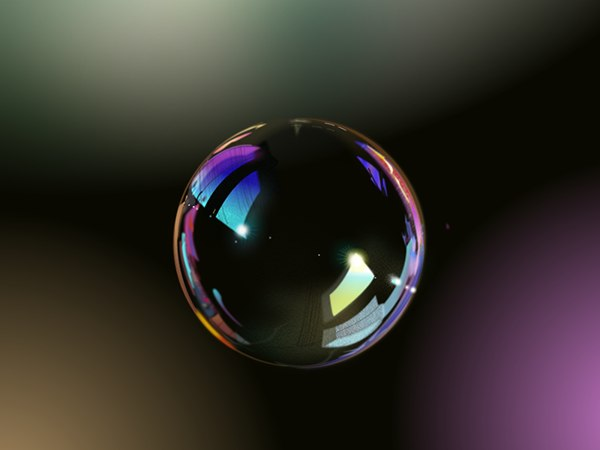
\includegraphics[width=0.5\textwidth]{img/soap_bubble.png}
	\caption{Мыльный пузырь с переливчатой поверхностью \cite{bubble_photo}}
	\label{fig:soap_bubble}
\end{figure}

Переливание возникает благодаря физическому явлению, называемому интерференцией в тонких плёнках \cite{interference}. 

Чтобы объяснить физику данного явления, необходимо ввести следующие понятия \cite{berne2000dynamic}:

\begin{itemize}[label=---]
    \item свет -- в физической оптике электромагнитное излучение, распространяемое в виде волны;
    \item световой луч (далее просто луч) -- линия, вдоль которой распространяется световая волна;
    \item фаза луча -- состояние волны в данный момент времени (функция координат и времени);
    \item длина волны -- расстояние между двумя ближайшими друг к другу точками в пространстве, в которых колебания происходят в одинаковой фазе;
    \item разность хода -- разница фаз между двумя волнами;
    \item интенсивность луча -- энергия, переносимая лучом в заданном направлении (от неё зависит яркость излучения).
\end{itemize}

На рисунке \ref{fig:interference} смоделирована интерференция в тонких плёнках.

Световой луч $B_1$ падает на внешний слой плёнки, от него отражается (луч $B_2$) и преломляется (луч $B_3$). В свою очередь на внутренний слой падает преломленный луч $B_3$ и так же отражается (луч $B_4$) и преломляется (луч $B_5$). После этого отражённый луч $B_4$ падает вновь на внешний слой, после чего отражается и преломляется (луч $B_6$). Лучи $B_2$ и $B_6$ оказываются параллельными, таким образом они будут взаимодействовать.

За счёт разности фаз лучей $B_2$ и $B_6$ суммарная интенсивность отличается от исходной и наблюдатель видит цвет, отличный от цвета источника \cite{interference}.

\begin{figure}[h]
	\centering
	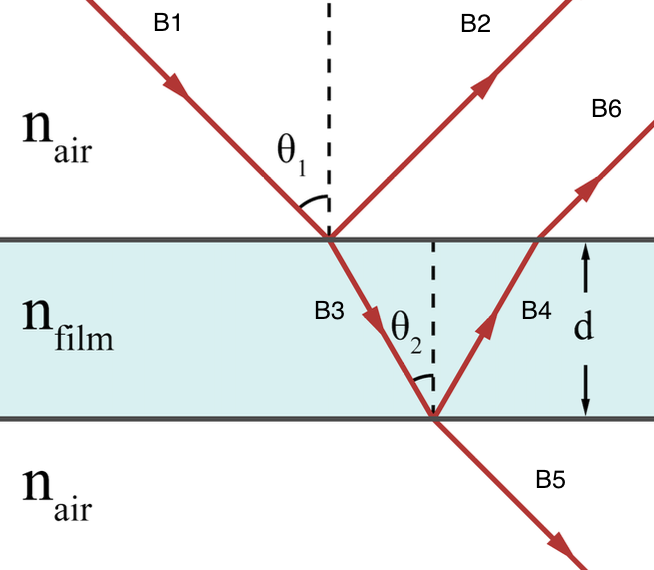
\includegraphics[width=0.4\textwidth]{img/interference.png}
	\caption{Интерференция в тонких плёнках \cite{berne2000dynamic}}
	\label{fig:interference}
\end{figure}

На рисунке \ref{fig:interference} присутствуют следующие обозначения:

\begin{itemize}[label=---]
    \item $n_{air}$ -- коэффицент преломления воздуха;
    \item $n_{film}$ -- коэффицент преломления мыльной воды;
    \item $\theta_1$ -- угол падения луча;
    \item $\theta_2$ -- угол преломления луча при вхождении в мыльную воду;
    \item $d$ -- расстояние между тонкими плёнками
\end{itemize}.


Пусть свет, поступающий вдоль $B_1$ имеет длину волны $\lambda$. Пленка имеет толщину $d$, а показатель преломления пленки равен $n_{film}$. Угол падения между $B_2$ и нормалью к поверхности равен $\theta_1$, а угол преломления -- $\theta_2$. Свет по лучу $B_6$ будет сдвинут по фазе относительно света по лучу $B_2$, а разность фаз будет определять, усиливают или гасят эти волны друг друга. Чтобы найти разность фаз, нужно сначала найти оптическую разность хода.

Свет всегда распространяется медленнее в более плотной среде, поэтому расстояние, пройденное светом в мыльной плёнке, нужно умножить на показатель преломления мыльной воды. Также когда свет переходит из одной среды в среду с более высоким показателем преломления, он претерпевает фазовый сдвиг, равный половине длины его волны. 

Разность хода $\Delta$ выражается следующим соотношением:
\begin{equation}
	\Delta = 2 \cdot d \cdot n_{film} \cdot \cos(\theta_2) - \frac{\lambda}{2}.
\end{equation}

Если в разность хода укладывается чётное число полуволн, то в точке падения луча будет максимум интенсивности света. Если в разность хода укладывается нечётное число полуволн, то в точке падения луча будет минимум интенсивности света.

Разность фаз $\delta$ выражается следующим соотношением:
\begin{equation}
	\delta = \frac{2 \cdot \pi \cdot \Delta}{\lambda}.
\end{equation}

Для волн с одинаковой интенсивностью итоговая интенсивность $I$ в результате интерференции выражается следующим соотношением:
\begin{equation}
	I = 2 \cdot I_0 \cdot (1 + \cos(\delta)).
\end{equation}

\clearpage


% =====================================================
\section{Формализация задачи}

На рисунке \ref{img:idef0_form} представлена формализованная задача.

\begin{figure}[h]
	\begin{center}
		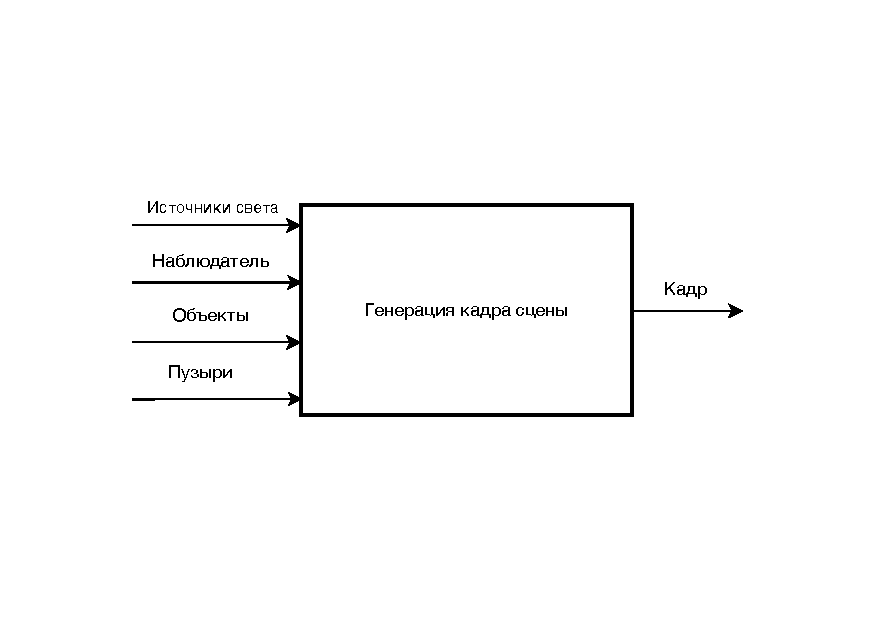
\includegraphics[width=\linewidth]{img/idef0_form.pdf}
	\end{center}
	\captionsetup{justification=centering}
	\caption{Формализованная задача с учётом выбранных алгоритмов}
	\label{img:idef0_form}
\end{figure}

% =====================================================
\section{Формализация объектов сцены}

На сцене могут присутствовать следующие типы объектов:
\begin{itemize}[label=---]
    \item источники света (задаются расположением и интенсивностью);
    \item наблюдатель (задаётся расположением и направлением взгляда);
    \item объекты (задаются моделью описания объектов, набором данных для данной модели, оптическими свойствами, являются выпуклыми);
    \item пузыри (задаются внешним и внутренним сфрическими слоями, оптическими свойствами).
\end{itemize}





% =====================================================
\section{Модели описания объектов}

Наиболее распространённые модели представления трёхмерных объектов в компьютерной графике: \textit{аналитическая}, \textit{полигональная}, \textit{воксельная}, \textit{равномерная сетка}, \textit{неравномерная сетка} \cite{piter_2002}, \cite{falcidieno2012modeling}, \cite{salomon2012computer}.

% -----------------------------------------------------
\subsection{Аналитическая модель}

Аналитической моделью называют описание поверхности с помощью математических формул, таких как $z = f(x, y)$ или $F(x, y, z) = 0$ \cite{piter_2002}.

Свойствами данной модели являются:
\begin{itemize}[label=---]
    \item возможность вычисления пересечения луча с объектом решением системы уравнений;
    \item возможность вычисления нормали в аналитическом виде при условии гладкости функции;
    \item необходимось составления объекта из нескольких поверхностей, если поверхность нельзя описать аналитически;
    \item возможность хранения только коэффициентов формул, задающих поврхности, при условии, что известен общий вид поверхностей;
    \item отсутствие погрешности при задании сферического объекта.
\end{itemize}



% -----------------------------------------------------
\subsection{Полигональная модель}

Для описания трёхмерных объектов в данной модели используются следующие элементы \cite{piter_2002}: 

\begin{itemize}[label=---]
    \item точка -- объект, размер которого не имеет значения;
    \item вектор -- объект, задаваемый двумя точками;
    \item полилиния -- объект, состоящий из векторов;
    \item полигон -- объект, имеющий площадь, ограниченную замкнутой полилинией;
    \item полигональная поверхность -- объект, состоящий из полигонов.
\end{itemize}

Свойствами данной модели являются:
\begin{itemize}[label=---]
    \item необходимость нахождения пересечения луча со всеми полигонами для поиска пересечения луча с объектом;
    \item необходимость вычисления нормали для каждого полигона;
    \item возможность описания объектов произвольной формы;
    \item присутствие погрешности при задании сферического объекта;
    \item необходимость хранения информации о каждом полигоне.
\end{itemize}



% -----------------------------------------------------
\subsection{Воксельная модель}

Воксельной моделью называют модель описания объектов в виде трехмерного массива кубических элементов \cite{piter_2002}.

Свойствами данной модели являются:
\begin{itemize}[label=---]
    \item необходимость нахождения пересечения луча со всеми гранями вокселей для поиска пересечения луча с объектом;
    \item необходимость вычисления нормалей для граней каждого вокселя;
    \item возможность описания объектов произвольной формы;
    \item присутствие погрешности при задании сферического объекта;
    \item необходимость хранения информации о каждом вокселе.
\end{itemize}



% -----------------------------------------------------
\subsection{Равномерная сетка}

Неравномерной сеткой называют модель описания поверхности в виде матрицы, каждый элемент которой хранит значение высоты узла сетки.

Свойствами данной модели являются:
\begin{itemize}[label=---]
    \item необходимость применения интерполяции для поиска пересечения луча с объектом;
    \item необходимость вычисления нормали для каждого узла относительно расположения окружающих его узлов;
    \item невозможность описания замкнутых объектов;
    \item присутствие погрешности при задании сферического объекта;
    \item необходимость хранения информации о каждом узле.
\end{itemize}



% -----------------------------------------------------
\subsection{Неравномерная сетка}

Неравномерной сеткой называют модель описания поверхности в виде множества отдельных точек, принадлежащих поверхности \cite{piter_2002}.

Свойствами данной модели являются:
\begin{itemize}[label=---]
    \item необходимость применения интерполяции для поиска пересечения луча с объектом;
    \item необходимость вычисления нормали для каждого узла относительно расположения окружающих его узлов;
    \item возможность описания замкнутых объектов;
    \item необходимость изменения расположения каждого узла для изменения геометрии объекта;
    \item необходимость хранения информации о каждом узле.
\end{itemize}



% -----------------------------------------------------

\subsection{Сравнение моделей описания объектов}

В таблице \ref{tbl:comparing_mod} представлены результаты сравнения моделей описания объектов и использованы следующие обозначения:

\begin{itemize}[label=---]
    \item А -- аналитическая модель;
    \item П -- полигональная модель;
    \item В -- воксельная модель;
    \item РС -- равномерная сетка;
    \item НС -- неравномерная сетка;
    \item N -- количество полигонов;
    \item M -- количество вокселей;
    \item K -- количество соседних троек точек.
\end{itemize}

\begin{table}[H]
	\begin{center}
        \small
		\caption{Сравнение моделей}
		\label{tbl:comparing_mod}
		\begin{tabular}{
              |m{3.4in}|
              >{\centering\arraybackslash}m{0.4in}|
              >{\centering\arraybackslash}m{0.4in}|
              >{\centering\arraybackslash}m{0.4in}|
              >{\centering\arraybackslash}m{0.4in}|
              >{\centering\arraybackslash}m{0.4in}|
              }
			 \hline
              & А & П & В & РС & НС \\
             \hline
             Временная сложность поиска нормали & $O(1)$ & $O(N)$ & $O(M)$ & $O(K)$ & $O(K)$ \\
             \hline
             Временная сложность поиска пересечения & $O(1)$ & $O(N)$ & $O(M)$ & $O(K)$ & $O(K)$ \\
             \hline
             Пространственная сложность хранения объектов & $O(1)$ & $O(N)$ & $O(M)$ & $O(K)$ & $O(K)$ \\
             \hline
             Возможность описания произвольных объектов & - & + & + & - & + \\
             \hline
             Отсутствие погрешности при задании сферического объекта & + & - & - & - & - \\
             \hline
		\end{tabular}
	\end{center}
\end{table}

По всем параметрам, кроме хранения произвольных объектов выигрывает аналитическая модель. Так как пузыри имеют сферическую форму, которую возможно описать аналитически, в работе использована аналитическая модель. Однако для демонстрации оптических свойств мыльных пузырей относительно других объектов, так же введена полигональная модель, так как она позволяет описывать объекты разных форм.

%=====================================================
\section{Модель освещения}

Модель освещения определяет интенсивность $I$ в каждой точке \cite{жаксылык2021применение}.

Наиболее распространёнными являются 2 модели освещения: \textit{локальная} и \textit{глобальная} \cite{будак2023сравнительный}, \cite{жаксылык2021применение}, \cite{боголепов2012система}, \cite{tomsk_2011}.

Локальная модель освещения рассматривает каждый объект отдельно и не учитывает взаимное расположение между ними \cite{жаксылык2021применение}. Так как для генерации мыльных пузырей необходимо учитывать взаимодействие между внешним и внутренним слоем мыльной плёнки для создания интерференции, данная модель освещения не подходит.

Глобальная модель освещения учитывает взаимное расположение между объектами, поэтому будет использоваться она \cite{будак2023сравнительный}, \cite{боголепов2012система}, \cite{tomsk_2011}.

Интенсивность $I$ в точке $P$ в глобальной модели освещения складывается из следующих компонент:

\begin{itemize}[label=---]
	\item фоновое освещение (ambient), существующее в любой области сцены и не зависящее от координат точки $P$ и источников света;
	\item рассеянный свет (diffuse), распространяющийся равномерно во все стороны при попадании на поверхность и зависящий от ориентация поверхности (нормали $N$), направления на каждый источник света $L$ и интенсивности источников света $I$;
	\item зеркальная составляющая (specular), зависящая от того, насколько близки направления на наблюдателя $V$ и отраженного луча $R$, интенсивности источников света $I$, а также учитывающая интенсивность отражённого луча $I_s$;
    \item преломлённая составляющая (refract), учитывающая интенсивность преломлённого луча $I_r$;
\end{itemize}

Тогда итоговая интенсивность в глобальной модели освещения рассчитывается следующим образом \cite{tomsk_2011}:

\begin{equation}
	I = k_aI_a + k_d\sum\limits_{j}^{}I_j(N \cdot L_j) + k_s\sum\limits_{j}^{}I_j(V \cdot R_j)^{\alpha} + k_sI_s + k_rI_r,
\end{equation}

где

    $k_a$ -- коэффициент фонового освещения;
    
    $k_d$ -- коэффициент диффузного отражения;
    
    $k_s$ -- коэффициент зеркального отражения;
    
    $k_r$ -- коэффициент пропускания;
    
    $I_a$ -- интенсивность фонового освещения;
    
    $I_j$ -- интенсивность $j$-го источника света;
    
    $I_s$ -- интенсивность отражённого луча;
    
    $I_r$ -- интенсивность преломлённого луча;
    
    $\vec{L_j}$ -- вектор, направленный к $j$-му источнику света;
    
    $\vec{N}$ -- вектор нормали в точке;
    
    $\vec{R}$ -- вектор отраженного луча;
    
    $\vec{V}$ -- вектор, направленный на наблюдателя;
    
    $\alpha$ -- коэффициент блеска.

\clearpage

%=====================================================
\section{Алгоритмы удаления невидимых линий и поверхностей}

Наиболее распространённые алгоритмы удаления невидимых линий и поверхностей: \textit{Робертса, с использованием Z-буфера, художника, Варнока, Вейлера~---~Азертона, трассировки лучей} \cite{devaifuture, warnock1969hidden, foley1996computer, кутенев2019разработка, половинина2018исследование, головнин2016базовые, tomsk_2011}.


% -----------------------------------------------------
\subsection{Алгоритм Робертса}

Этапы алгоритма Робертса \cite{tomsk_2011}:
\begin{enumerate}[label=\arabic*)]
    \item Определить грани тела, перекрываемые самим телом. 
    \item Определить рёбера, перекрываемые другими телами.
    \item В случае наличия перекрытия найти видимую часть ребра.
\end{enumerate}

Работа с гранями и рёбрами говорит о том, что данный алгоритм можно использовать только для тел, заданных полигональной моделью.

Временная сложность алгоритма равна $O(N^2)$, где $N$ -- количество граней.



% -----------------------------------------------------
\subsection{Алгоритм с использованием z-буфера}

В алгоритме с использованием z-буфера, есть \textit{буфер кадра} ($frame\_buf$), хранящий интенсивность для каждого пикселя и \textit{z-буфер} ($z\_buf$), хранящий глубину видимого пикселя.

Этапы алгоритма с использованием z-буфера  \cite{tomsk_2011}:
\begin{enumerate}[label=\arabic*)]
    \item Заполнить $frame\_buf$ фоновым значением интенсивности. 
    \item Заполнить $z\_buf$ минимальным значением $z$.
    \item Преобразовать каждое тело в растровую форму.
    \item Для каждого пикселя $(x, y)$ в теле вычислить его глубину $z(x, y)$.
    \item Сравнить глубину $z(x, y)$ со значением $z\_buf(x, y)$.
    \item Если $z(x, y) > z\_buf(x, y)$, то записать атрибут этого тела (интенсивность, цвет и т. д.) в $frame\_buf(x, y)$ и заменить $z\_buf(x, y)$ на $z(x, y)$. В противном случае никаких действий не производить.
\end{enumerate}

Данный алгоритм можно использовать для обработки как аналитически заданных тел, так и для тел, заданных полигональной моделью.

Так как размер экрана ограничен, временная сложность алгоритма равна $O(WHN)$, где $W$ -- ширина экрана в пикселях, $H$ -- высота экрана в пикселях, $N$ -- количество граней и аналитических поверхностей.


% -----------------------------------------------------
\subsection{Алгоритм художника}

Этапы алгоритма алгоритма художника \cite{tomsk_2011}:

\begin{enumerate}[label=\arabic*)]
    \item Отсортировать грани по глубине (от дальней до ближайшей к наблюдателю). 
    \item Отрисовать грани в отсортированном порядке.
\end{enumerate}

Данный алгоритм не справляется с циклическим перекрытием тел друг друга. Кроме того, необходимо учитывать неоднозначность выбора порядка сортировки.

Так как алгоритм работает с гранями, его можно использовать только для тел, заданных полигональной моделью.

Сложность алгоритма равна $O(N)$, где $N$ -- количество граней, однако необходимо также учитывать предварительную сортировку.


% -----------------------------------------------------
\subsection{Алгоритм Варнока}

В алгоритме Варнока используется прямоугольная область, которая изначально равна размеру экрана. В ходе работы алгоритма область может разбиться на 4 равые части, потом каждая часть аналогично рассматривается отдельно и может разбиться ещё на 4 равные части и так далее.

Этапы алгоритма Варнока \cite{warnock1969hidden}:

\begin{enumerate}[label=\arabic*)]
    \item Проверить область на соответствие каждому из случаев:
    \begin{itemize}[label=---]
        \item Проекция ни одной грани не попадает в область, тогда закрасить область цветом фона.
        \item Проекция только одной грани содержится в области или пересекает её, тогда закрасить проекцию грани, а остальное закарсить цветом фона.
        \item Существует грань, проекция которой полностью накрывает данную область, и эта грань расположена к картинной плоскости ближе, чем все остальные грани, проекции которых пересекают данную область, тогда закрасить область цветом данной грани.
    \end{itemize}
    \item Если область не соответствует ни одному пункту, то разбить её на 4 части и повторить предыдущие шаги.
\end{enumerate}

Так как алгоритм работает с гранями, его можно использовать только для тел, заданных полигональной моделью.

Временная сложность алгоритма равна $O(WHN)$, где $W$ -- ширина экрана в пикселях, $H$ -- высота экрана в пикселях, $N$ -- количество граней.



% -----------------------------------------------------
\subsection{Алгоритм Вейлера~---~Азертона}

Этапы алгоритма Вейлера~---~Азертона \cite{tomsk_2011}:

\begin{enumerate}[label=\arabic*)]
    \item Отсортировать грани по глубине (от дальней до ближайшей к наблюдателю). 
    \item Из списка выбирается ближайшая грань и по границам её проекции остальные грани разбиваются на части, которые лежат полностью внутри ($F_in$) выбранной грани или снаружи ($F_{out}$) её.
    \item Если в $F_{in}$ есть части, которые ближе текущей грани (циклическое экранирование), тогда каждая такая часть используется для разбиения всех граней из множества $F_{in}$.
    \item Повторить предыдущие шаги с $F_{out}$.
\end{enumerate}

Так как алгоритм работает с гранями, его можно использовать только для тел, заданных полигональной моделью.

Временная сложность алгоритма равна $O(N^2)$, где $N$ -- количество граней.



% -----------------------------------------------------
\subsection{Алгоритм трассировки лучей}

Идея, лежащая в основе алгоритма трассировки лучей, заключается в том, что наблюдатель видит любой объект посредством испускаемого неким источником света лучом, который падает на этот объект и затем доходит до наблюдателя. Однако обычно используют алгоритм обратной трассировки лучей, в котором лучи пускаются от наблюдателя до источника света \cite{tomsk_2011}.

Этапы алгоритма трассировки лучей для каждого пикселя:
\begin{enumerate}[label=\arabic*)]
    \item Найти уравнение трассируемого луча, проходящего через рассматриваемый пиксель и положение взгляда наблюдателя.
    \item Найти точку пересечения луча с ближайшим объектом сцены, закрасить пиксель цветом данного объекта и перейти к следующему пикселю.
    \item Если нет пересечений, то закрасить пиксель цветом фона и перейти к следующему пикселю.
\end{enumerate}

Данный алгоритм позволяет учесть преломления и отражения. Для этого необходимо не останавливаться на достижении лучом объекта, а трассировать отражённый и преломлённый лучи.

Данный алгоритм можно использовать для обработки как аналитически заданных тел, так и для тел, заданных полигональной моделью.

Сложность алгоритма равна $O(WHN)$, где $W$ -- ширина экрана в пикселях, $H$ -- высота экрана в пикселях, $N$ -- количество граней и аналитических поверхностей..


\clearpage

% -----------------------------------------------------
\subsection{Сравнение алгоритмов}

В таблице \ref{tbl:comparing_algo} представлены результаты сравнения алгоритмов и использованы следующие обозначения:

\begin{itemize}[label=---]
    \item Р -- алгоритм Робертса;
    \item ЗБ -- алгоритм с использованием z-буфера;
    \item Х -- алгоритм художника;
    \item В -- алгоритм Варнока;
    \item ВА -- алгоритм Вейлера~---~Азертона;
    \item ОТ -- алгоритм обратной трассировки лучей;
    \item $W$ -- ширина изображения в пикселях;
    \item $H$ -- высота изображения в пикселях;
    \item $N$ -- количество граней и аналитических поверхностей.
\end{itemize}

\begin{table}[h]
	\begin{center}
        \small
		\caption{Сравнение алгоритмов}
		\label{tbl:comparing_algo}
		\begin{tabular}{
              |m{1.3in}|
              >{\centering\arraybackslash}m{0.7in}|
              >{\centering\arraybackslash}m{0.7in}|
              >{\centering\arraybackslash}m{0.7in}|
              >{\centering\arraybackslash}m{0.7in}|
              >{\centering\arraybackslash}m{0.7in}|
              >{\centering\arraybackslash}m{0.7in}|
              }
			 \hline
              & Р & ЗБ & Х & В & ВА & ОТ \\
             \hline
             Возможность построения отражений и преломлений & - & - & - & - & - & + \\
             \hline
             Возможность использования без сортировки & + & + & - & + & - & + \\
             \hline
             Возможность использования для аналитических объектов & - & + & - & - & - & + \\
             \hline
             Временная сложность & $O(N^2)$ & $O(WHN)$ & $O(N)$ & $O(WHN)$ & $O(N^2)$ & $O(WHN)$ \\
             \hline
		\end{tabular}
	\end{center}
\end{table}

Только алгоритм обратной трассировки лучей (далее трассировки лучей) позволяет реализовать отражение и преломление, может работать с объектами, заданными аналитически, а также учитывать глобальную модель освещения, поэтому в данной работе будет использован именно он, хотя он не является самым эффективным из рассмотренных алгоритмов.

% =====================================================
\section{Построение теней}

Алгоритмы затенения в случае точечных источников света идентичны алгоритмам удаления невидимых линий и поверхностей, однако точка наблюдения перемещается в источник света \cite{crow1977shadow}, \cite{романюк2000алгоритмы}. Тогда точки, невидимые из источников света, являются затенёнными.

Так как был выбран алгоритм трассировки лучей, можно использовать его и для поиска теней. В отличие от задачи удаления невидимых линий и поверхностей, для построения теней луч пускается от рассматриваемой точки до источника света. При наличии объектов на пути луча, даннная точка затенена.

\clearpage

% =====================================================
\section{Формализация задачи с учётом выбранных алгоритмов}

На рисунке \ref{img:idef0_form_algo} представлена формализованная задача с учётом выбранных алгоритмов.

\begin{figure}[h]
	\begin{center}
		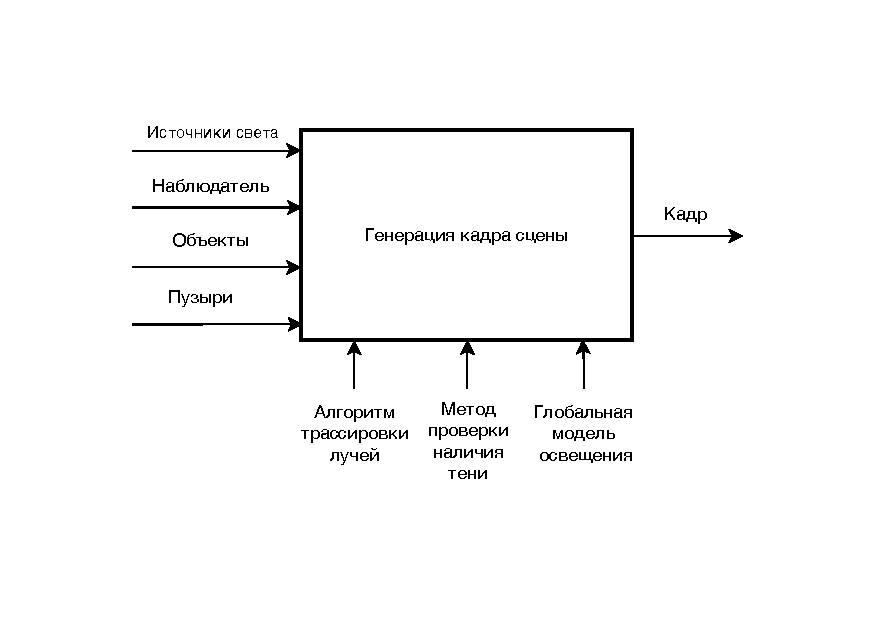
\includegraphics[width=\linewidth]{img/idef0_form_algo.pdf}
	\end{center}
	\captionsetup{justification=centering}
	\caption{Формализованная задача с учётом выбранных алгоритмов}
	\label{img:idef0_form_algo}
\end{figure}


%=====================================================
\section{Выводы из аналитической части}

В аналитической части была представлена физическая модель мыльных пузырей, проанализированы модели представления объектов и алгоритмы решения основных задач компьютерной графики. По результатам проведённого анализа были выбраны аналитическая и полигональная модели представления объектов и алгоритм трассировки лучей для удаления невидимых линий и поверхностей и построения теней.

